%===================================== CHAPTER 8 Implementation =================================

\chapter{Implementation}

This chapter discusses the details of the system implementation process, both for front end and for back end.

\section{Front end}

\subsection{User interface}

Early on in development, the team discovered several limitations of the Ionic framework. For example when using a list to display stories, it was not possible to swipe the list both left and right. The idea was to swipe one way to add a story to be read later, and swipe the other way to reject a story from the list entirely.  Because this proved to be impossible, the views were redesigned into a different solution which was much less based around swiping.\newline

As this is an application for mobile devices, it had to be adapted to work on different screen sizes. The team found that it would most likely be best to target a relatively small screen size and then simply enlarge it for bigger screens. This eliminated the issue of having to compress the components to fit smaller screen sizes and potentially be forced to redesign the whole view to fit small screens.\newline

The applications uses many different icons in various parts of the interface, and these have been the source of much debate and redesign. The icons used to represent categories were not always understood by users, and some categories like “local tradition and food” were difficult to represent universally with just a single icon. Also the bookmark icon shown in the upper right area of figure 8.xx was confusing to many users, and there was a concern in the team that this icon might not accurately represent that it allows the user to save the story in a collection.\newline

Adopting accurate naming conventions for the different components has also been a considerable issue. Stories can be saved in collections, but these collections have interchangeably been called lists, tags, and bookmarks in the system. Also when asking a user to input their preferred categories to receive stories from, there has been some confusion because of interchangeably calling these categories for interests,  preferences, and categories.\newline

Implementing media, and especially video, has been a challenge in the project. An issue with this has been that playing videos is handled differently on iOS and Android, which had resulted in some bugs that only appear on one platform and not the other. These types of issues have been problematic to fix and has taken up much time to fix. In addition, the videos provided by the Digitalt fortalt website come from different sources. Some of them are Youtube videos, others are Vimeo videos, and there are also other variations. Integrating all these different formats smoothly into the application has been a challenge in itself.

\subsection{Prototype}

The prototype has been through multiple iterations. Early on, it was imagined to have a sort of “magic” discovery function where a user would for example rub a crystal ball and receive a recommended story. This idea was later discarded because the team decided it would be better usability to present the user with multiple recommended story that they could simply browse through instead.\newline

Another of the early ideas was for the user to receive a “daily story” or some sort of schedule for being presented with recommended stories. However, due to workload and time constraints, this requirement was heavily down prioritized. The most important parts were the personalization and usability aspects, so receiving notifications seemed like an unnecessary extra feature.\newline

A big issue for the interface design has been the handling of the different media elements (text, pictures, audio, video) and how these should be positioned relative to each other. For a while the team designed the application to have one tab for each of these four elements in the story view, as shown to the left in figure 8.XX. The customer had a concern that this might not be the optimal solution, as a user would for example not be able to read text and view pictures simultaneously. After some discussion, the interface was redesigned so that the text would be persistent, and instead the user could tab between pictures, audio, and video. The resulting design can be seen to the right in \textbf{Fig \ref{prototype}}. 

\begin{figure}
	\centering
	\begin{subfigure}[h]{0.4\textwidth}
		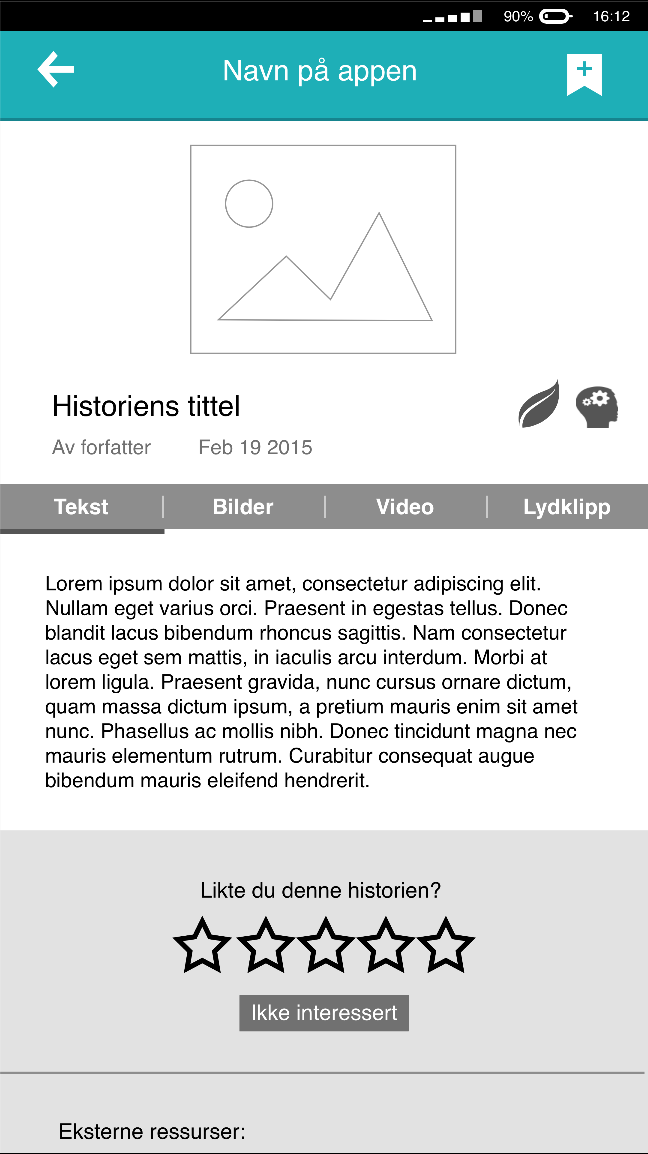
\includegraphics[width=\textwidth]{fig/prototype1}
	\end{subfigure}
	%
	\begin{subfigure}[h]{0.4\textwidth}
		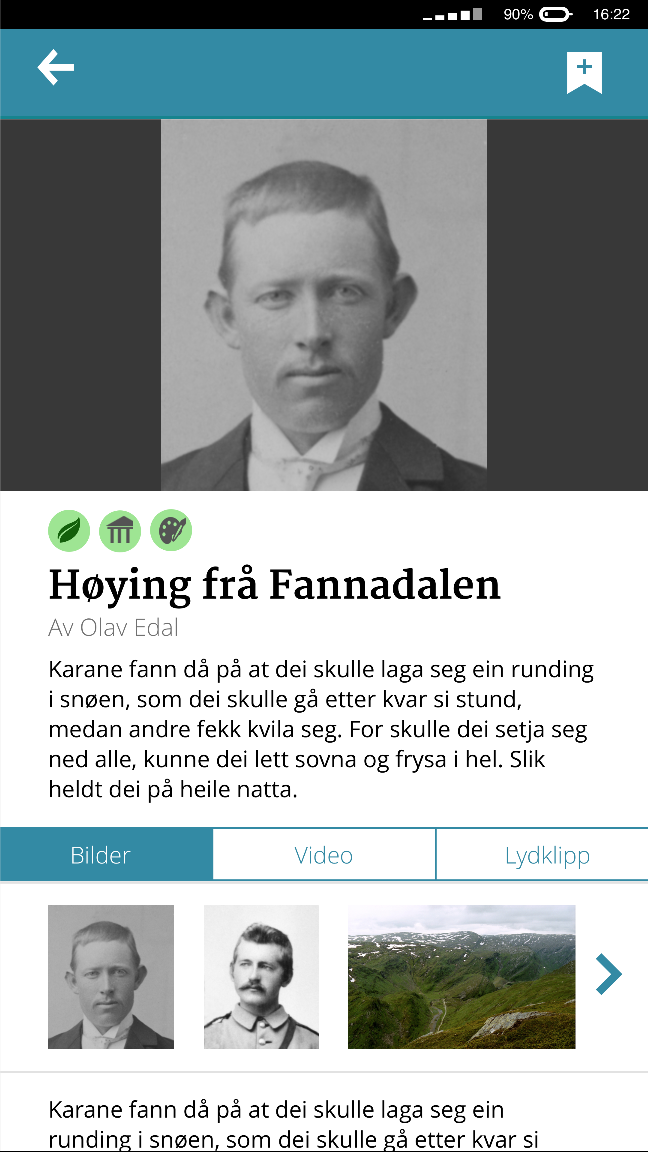
\includegraphics[width=\textwidth]{fig/prototype2}
	\end{subfigure}
	\caption{Comparison of the story view in the first and second version of the prototype.}
	\label{prototype}
\end{figure}

\section{Back end}

This section describe the development of each part of the back end. It aims to give a timeline of the development and explain how and why important decisions were made. The different parts described here are the database, personalization and the communication between front end and back end. 

\subsection{Database}

Based on the first version of the functional requirements for the application an initial ER-diagram was made in the middle of february. At this stage the customer and the team had not come to an agreement on a prioritization of the non-functional requirements. This meant that there for instance was not clear how important the performance of the system would be for the customer, an attribute of the system which would influence how much info should be stored for each story in the database versus have much info should be retrieved from Digitalt fortalt every time a user views a story. However, the changes to the initial diagram have been relatively minor. Some of the alterations were based on updated requirements from the customer, while others stem from the group and are optimization of the data model or changes made to facilitate the personalization. \newline

Shortly after the first ER-diagram was made, an SQL-script for creating a database was also made. Since the ER-diagram has undergone changes for quite some time after the first version was made, these changes has also influenced the SQL-script. This means that a change in the data model have lead to more work than just updating the ER-diagram. However, the progress of the project relied on testing against an operational database, for instance regarding the harvesting of stories from Digitalt fortalt. \newline

The customer had early on said that the retrieval of research data about the use of the application was important for them. Initially, the details of this was not properly formulated and the initial data model therefore did not reflect this. After receiving a detailed list from the customer describing the research data to be gathered, alterations - mostly additions - in the data model were made to accommodate this. This concerned storing timestamps for user actions and states of stories.  \newline

The team did not decide or understand how to do the personalization until mid March. This decision introduced changes to existing tables and the need to create additional tables and views in the database. Mahout had requirements for the input data, which meant that a view was created to store all the necessary data for collaborative filtering. Using this view made it straightforward to put the desired data from the database into Mahouts data model.

\subsection{Personalization}

The way personalization was implemented was by having the user give their preferences about which types of stories they enjoy, and also by harvesting circumstantial  information about the user in order to provide relevant stories. Users of this system are also allowed to give feedback on the recommendation of stories from the database to achieve further personalization.  Users receive story recommendations based on other users’ preferences and recommendations, i.e. collaborative filtering. The system was developed as a client/server architecture, while the database containing the stories was provided by Digitalt fortalt [es19]. The stories are found in a variety of formats such as text, images, audio and video.

\subsection{Front end - back end communication}

Communication between front end and back end was handled using http post requests.
AngularJs \$http is a core service for reading data from remote servers, which is called every time the application needs to add, retrieve, update or delete data. When an http request is made four fields are set: method, headers, url and data. The method field determines the http request method, which in this application is set to post, and the headers field sets the content type to JSON. The url is the location of the remote server script that handles http requests. In the data field the action to be executed is specified, in addition to any data needed to perform the desired action.\newline

Each http request is managed by the same back end php script. This script decodes the http request, determines which action to perform and executes it. When the script has finished executing, a json response is returned to front end with the desired data.

\cleardoublepage